\begin{pastexam}[label={px:gw3-109-ds-03}]{關務三等資訊處理 109 年 第三題}
（申論；20 分）

新冠肺炎肆虐全球，目前世界各國生物及醫學實驗室均在尋找新型冠狀病毒的基因，假設新型冠狀病毒的基因由 A, T, C, G, H, M 核苷酸所組成，今有一新型冠狀病毒的基因為 ATATATCCHCGMCMA，請使用霍夫曼演算法（Huffman Algorithm）設計霍夫曼樹（Huffman Trees），並設計出一編碼表（Code Words），依序分別寫出 A, T, C, G, H, M 核苷酸的編碼位元數，將此新型冠狀病毒基因以最少位元數（Minimum Bit Strings）編碼，並計算出最少位元數（Minimum Bit Strings）。（20 分）
\end{pastexam}

\begin{pastsoln}
答案：A、T、C 各 $2$ 位元，G、H 各 $4$ 位元，M $3$ 位元；最少 $36$ 位元。

霍夫曼演算法見資結書第~19.3~節，做法同 歷屆試題~\ref{px:gk3-096-ds-02}。

\textbf{數次數}。 ATATATCCHCGMCMA 共 $15$ 個字母：
\begin{center}
\begin{tabular}{l*{6}{c}c}
\toprule
字母 & A & T & C & G & H & M & 合計 \\
\midrule
次數 & 4 & 3 & 4 & 1 & 1 & 2 & 15 \\
\bottomrule
\end{tabular}
\end{center}
（A 在第 1、3、5、15 個；T 在第 2、4、6 個；C 在第 7、8、10、13 個；H 第 9 個；G 第 11 個；M 第 12、14 個。）

\textbf{建霍夫曼樹}。 每次取出最小的兩棵合併（小的放左邊、記 $0$）。 權重相同時，先取單一字母、再取合併出來的樹，單一字母之間依題目的順序
A, T, C, G, H, M：
\begin{center}
\begin{tabular}{clc}
\toprule
步驟 & 取出的兩棵 & 新樹權重 \\
\midrule
1 & G 1、H 1 & 2 \\
2 & M 2、$\{$GH$\}$ 2 & 4 \\
3 & T 3、A 4 & 7 \\
4 & C 4、$\{$MGH$\}$ 4 & 8 \\
5 & $\{$TA$\}$ 7、$\{$CMGH$\}$ 8 & 15 \\
\bottomrule
\end{tabular}
\end{center}
\begin{center}
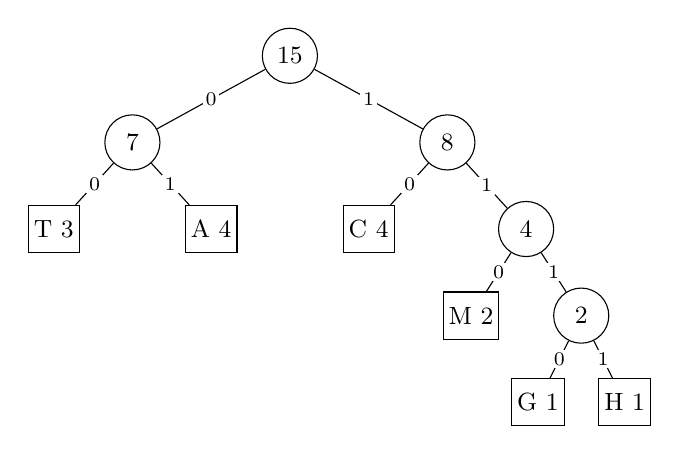
\begin{tikzpicture}[level distance=11mm,
  level 1/.style={sibling distance=40mm},level 2/.style={sibling distance=20mm},
  level 3/.style={sibling distance=14mm},level 4/.style={sibling distance=11mm},
  every node/.style={font=\small},
  iv/.style={circle,draw,inner sep=1pt,minimum size=7mm},
  lf/.style={rectangle,draw,inner sep=2pt,minimum height=6mm},
  e/.style={font=\scriptsize,fill=white,inner sep=1pt}]
\node[iv] {15}
  child {node[iv] {7}
    child {node[lf] {T 3} edge from parent node[e] {0}}
    child {node[lf] {A 4} edge from parent node[e] {1}}
    edge from parent node[e] {0}}
  child {node[iv] {8}
    child {node[lf] {C 4} edge from parent node[e] {0}}
    child {node[iv] {4}
      child {node[lf] {M 2} edge from parent node[e] {0}}
      child {node[iv] {2}
        child {node[lf] {G 1} edge from parent node[e] {0}}
        child {node[lf] {H 1} edge from parent node[e] {1}}
        edge from parent node[e] {1}}
      edge from parent node[e] {1}}
    edge from parent node[e] {1}};
\end{tikzpicture}
\end{center}

\textbf{編碼表}（依題目順序）：
\begin{center}
\begin{tabular}{l*{6}{c}}
\toprule
核苷酸 & A & T & C & G & H & M \\
\midrule
編碼 & 01 & 00 & 10 & 1110 & 1111 & 110 \\
位元數 & 2 & 2 & 2 & 4 & 4 & 3 \\
\bottomrule
\end{tabular}
\end{center}

\textbf{編碼結果}：A T A T A T C C H C G M C M A 依序換成碼：
\[
\texttt{01\,00\,01\,00\,01\,00\,10\,10\,1111\,10\,1110\,110\,10\,110\,01}
\]
\textbf{最少位元數}：$4 \times 2 + 3 \times 2 + 4 \times 2 + 1 \times 4 + 1 \times 4 + 2 \times 3 = 8 + 6 + 8 + 4 + 4 + 6 = 36$ 位元。 霍夫曼碼是
最佳前置碼（資結書定理~19.5），所以 $36$ 是用前置碼逐字母編碼時的最少位元數。 對照：$6$ 種字母用定長碼要 $3$ 位元，共 $45$ 位元。

\textbf{平手的處理}。 第 3 步時 T 3 要和三個權重 $4$ 的（A、C、$\{$MGH$\}$）之一合併，選哪一個樹形就不同，碼也會不同；但每一種選法得到的碼長都是
A、T、C 各 $2$、M $3$、G、H 各 $4$（例如 T 和 $\{$MGH$\}$ 合併時，A、C 合成一棵，T 深度 $2$，M 深度 $3$，G、H 深度 $4$），總位元數一定是 $36$。
\end{pastsoln}
